
%Chapter 1

\renewcommand{\thechapter}{1}

\chapter{Introduction}


%We must proceed in life as kittens... into the box, out of the box, pause, into the box again, then out of the box just in time for more food...

A few centuries ago one of the greatest strides in astronomy was made by Kepler working off Tyco Brahe's data in understanding planetary orbits. Keplar had discovered that planets move along elliptical orbits with the sun at one of the foci and thus developed the laws of planetary motion. In 1609 the concept was revolutionary yet it raised a more interesting question, why do planets move in elliptical orbits? Kepler said that each planet was guided in its elliptical orbit by a resident angel, the model still needed refinement. 
Two hundred and fifty years later, another significant discovery was made on the nature of light by James Maxwell. Apparently, the light from mars shining into Tyco Brahe's naked eye (He did not use a telescope) had propagated through space as an electro magnetic wave. The propagation of light through a vacuum would require electric fields without the presence of charge, thus it was proposed that the universe is filled with aether through which electromagnetic waves could propagate. 

Fast forward to the era of the standard model, and  precision cosmology . The standard model provides as a nearly perfect framework to understand the interactions of particles we know of. Precision cosmological measurements are now constraining parameters deemed impossible several decades ago (Plank is a huge step up from Tyco's eye ball), and has provided the basis for the concordance cosmological model ($\rm \Lambda CDM$). Apart from knowing that planets move in elliptical orbits we also know that the universe is primarily composed of dark energy (69.2\%) and dark matter (25.8\%). Ordinary particles described by the standard model which compose our current understanding of `everything' only constitute 4.82\% of the universe.
%We have achieved a great strides measuring precisely that we are surrounded by five times more mass than the ordinary matter which we can see or feel. Raising the standard four year old questions, why?, where?, when?, what is it? The first we disregard as an impossibility to answer. The leading theories indicate that dark matter is gravitationally bound and distributed in a halo like structure around galaxies but we can't definitively answer that until we can detect it. When is now. A leading candidate for dark matter is a particle which carries mass and only couples gravitationally and hopefully couples the elctroweak force so that we can have a chance of ever directly observing it.  

%We proceed with exploring the box, after having feasted.... a century from now will seem like kittens trapped in a box, playing with xenon, leaving behind only a mass underground Unicorn art galleries in Lead SD?... we were here searching for dark matter, TS dump, bolt seized, ACRS forced xenon recovery, slow control computer crash, the DAQ is shooting lighting bolts (over a hundred unicorns drawing are posed in the underground control room ...and counting)

\section{Outline of Thesis}

In this section we review current cosmological evidence for the existence of dark matter, and give an overview of dark matter candidates along with the WIMP model. We also review if WIMPs existes how they could be detected and the and how scattering off a nuclei would look.

In Chap.\ 2, We overview the LUX detector, a liquid xenon time projection chamber (TPC), and how it searchers for WIMPs. We conclude the chapter with the most recent LUX science results which holds the worlds leading limit for spin independent WIMP nucleon scattering cross section.

In Chap.\ 3, the position dependent corrections of energy deposition in the LUX detector are discussed.

In Chap.\ 4, the absolute energy scale calibration of the LUX detector is discussed.

Chapter 5 provides the conclusion to the thesis.

\section{Evidence for Dark Matter}

Astronomical observations hinting at the existence of dark matter were first observed in 1932 by Oort \cite{Oort} and more precisely in 1937 by Zwicky  \cite{Zwicky}. Both noted discrepancies in galactic mass measurements when comparing the luminous mass and the mass attained from galactic rotation curves measured by red shifts. Oort had noted up to a factor of ten more mass than luminous mass in the Sombrero Galaxy and Zwicky found a factor of 500 for the Coma cluster. Both the observations were far to large to be accounted for by light absorption, indicating the existence of dark matter to account for the missing mass. Since then more evidence for the existence of dark matter has been compiled, including big ban nucleosynthesis (BBN), anisotropies in the cosmic microwave background (CMB), formation of large structures, galactic ration curves, and gravitational lensing. All independent techniques leading to a unified conclusion for the existence of non baryonic and non luminous matter. Individually some pieces of evidence, such as galactic rotation curves, can be explained by modifications to general relativity (GR), but not all simultaneously. The existence of non relativistic, dark matter particles are required unify all known observations. This dark matter does not couple to the electromagnetic force and is thus able to avoid our standard detection techniques, making its presence felt on large scales via gravity. In the last thirty years significant progress has been made in the direct detection of such a particle, the forefront of which will be presented in this thesis.

\subsection{Galactic Rotation Curves}

There are two common methods for measuring the mass of a galaxy or cluster of galaxies. First, one can use the total luminosity and the known distance to the galaxy to determine the luminous mass, that is the mass corresponding to the visible light. Second, the rotational velocities of stars orbiting the galactic center can be mapped and used to determine the mass distribution as a function of galactic radius. Rotational velocities of stars around galactic centers at large distances can be measured with Doppler shift, with more recent measurement relying on the 21 cm H1 line from hydrogen as the standard candle. The rotational velocities of objects orbiting galaxies are highly non relativistic moving at speeds on the order 100 km/s. At the outer edges of the luminous galactic centers, typically past 5 kpc the velocity distribution is expected to fall off as redacted by Newtonian mechanics $\sim$1/r. Yet observations from as early as 1932 indicate that velocity distributions tend to remain constant with radius suggesting that the objects are not rotating around the central luminous mass, rather they are rotating inside a solid body of dark matter \cite{Oort} \cite{Zwicky} \cite{Galactic_Velocities} \cite{DarkMatter_MW}. The velocity distributions measured for the Milky Way galaxy are show in \ref{fig:MW_Rotation}.

\begin{figure}[h!]\centering
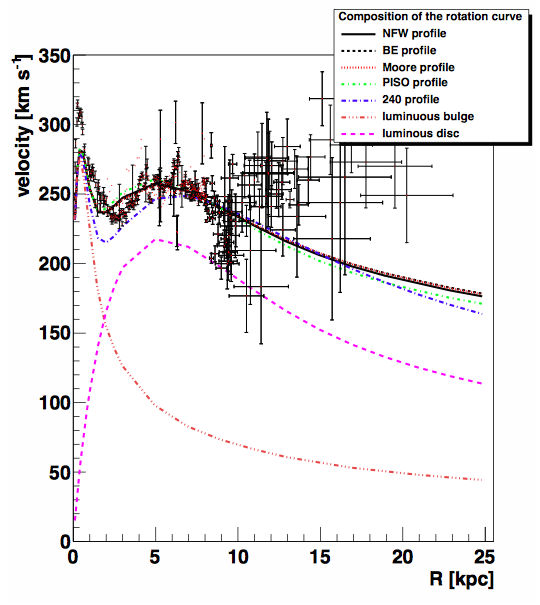
\includegraphics[width=80mm]{Intro/Ch1_Figures/MW_Rotation.png}
\caption{Measured rotational velocities vs. radius in the Milky Way galaxy. The velocity distribution is consistent with a halo of mass surrounding the galaxy well beyond the observed luminous disk \cite{DarkMatter_MW}. }
\label{fig:MW_Rotation}
\end{figure}

\subsection{BBN}

Big band nucleosynthesis (BBN) accounts for the relative abundances of light elements in the universe today, including H, D, $\rm He^3$, $\rm He^4$ and $\rm Li^7$ \cite{BBN}. BBN took place in a relatively short time window several seconds after the big bang when the universe cooled below $\rm10^{11}$K (10 MeV) and seized as the temperature cooled below $\rm10^9$K (100 keV). Under the temperature conditions of BBN it was energetically favorable for free protons and neutrons to undergo nuclear fusion and is the only mechanism to produce light elements we see today. The heavier elements were later fused together in stars and ejected upon the star's death into the cosmos. Nuclear cross sections of protons, neutrons and light elements have been measured to high person and can be combined with the expansion rate of the universe to precisely predict the relic abundances of baryonic matter. Observations constrain the abundances of the light elements to be H$\sim$ 75\%, D$\sim$ 25\%, $\rm He^4$ $\sim$ 0.01\%, $\rm Li^7$ $\sim 10^{-10}$ \%. The ratio of D/H has been used to constrain the relic density of baryonic matter to be $\Omega_b h^2$= 0.02202 $\pm$ 0.00046 \cite{OmegaB_BBN}.

\begin{equation}
\centering
\Omega_b h^2= \frac{p_b}{p_c}
\end{equation}

\noindent Where h is the Hubble constant H dividend by 100 ($\rm H_0/100$), $p_b$ is the baryonic density and $p_c$ is the critical density required for a flat universe (verified by the CMB). We can write the $\rm i^{th}$ density component as: 

\begin{equation}
\centering
\Omega_i \equiv \frac{p_b}{p_c} = \frac{8\pi G \rho_i}{3H^2}
\end{equation}

\noindent Where G is the gravitational constant, H is the Hubble constant (found in table \ref{table:Cosmo_Param}). 

The baryon density measured using BBN is constrained to within 1\% and in agreement with the latest constraints from Plank's CMB data, $\Omega_b h^2$= 0.02205 $\pm$ 0.00028 \cite{Planck_Param}.

\subsection{CMB}

The early universe consisted of a plasma making the universe opaque to photons as they scattered off free electrons. As the temperature fell below the binding energy of hydrogen 13.6 eV, electrons settled in to form neutral atoms and the universe became transparent to its own light. The mean temperature of decoupling was actually at 0.25 eV ($\sim 4000 \, K$ as photons still scatter frequently near the binding energy of hydrogen \cite{BBN}. The cosmic microwave background (CMB) emanated from this time after making a final scatter photons decoupled from electrons effectively attaining a mean free path on the scale of the universe. Thus photons observed today at the red shift temperature of 2.72548$\pm$0.00057 K \cite{CMB_Temp} have not interacted from the time of last scatter 379,000 years after the bing bang.

%photons and baryons were tightly coupled together in a plasma

%Image of Cobe, WMAP, Plank
NASA/JPL-Caltech/ESA


\begin{table}[h!]
\footnotesize
\begin{center}
\begin{tabular}{|c|c|c|c|c|c|}
\hline
Parameter & Value & Definition\\ \hline
$\Omega_bh^2 $ 		& 0.2214$\pm$0.00024 		&Baryon energy density \\ \hline
$\Omega_ch^2 $ 		& 0.1187$\pm$0.0017			& Cold dark matter energy density\\ \hline
$\Omega_mh^2 $ 		& 0.1423$\pm$0.0029 $^*$ 	& Total matter energy density\\ \hline
$\Omega_{\Lambda}$& 0.692 $\pm$ 0.010			&  Dark energy density \\ \hline
$\Omega_K$ 			& -0.0005$\pm$0.0065 (95\%) & Curvature\\ \hline
$\Sigma_{m_v}$		& $<$ 0.230 					& Sum of neutrino masses [eV] \\ \hline
$H_0$ 					& 67.77$\pm$0.77				& Hubble Constant [$\rm km s^{-1} Mpc^{-1}$]\\ \hline
\end{tabular}
\caption{Cosmological parameters. $^*$ Only Planck}
\label{table:Cosmo_Param}
\end{center}
\end{table}

\subsection{BAO}
Sloan result

\subsection{Gravitational Lensing}

At large distances the velocity of objects around the center of a galaxy does not fall off as predicted by Newtonian physics. Instead the velocity distributions appear constant as if a halo of �non-luminous mass was surrounding the galaxy. The rotation curve of our own Milky-way galaxy requires the presence of dark-matter [14]. Astronomical observations of the bullet-cluster also support the existence of dark-matter. The bullet-cluster is made up of two galaxy clusters which have recently collided and passed through each other. The collision has caused the ordinary matter to heat and emit X-rays, from elector-magnetic interactions, allowing for the mass distribution to be mapped [15]. However, the observed concentration of mass is not consistent with the center of mass predicted by GR, specifically gravitational lensing [16]. The way light bends around the bullet-cluster would indicate the presence of a dark-matter shell which, unlike the ordinary matter, has passed through at a faster rate due to the lack of interactions. Figure 3 shows the concentration of mass in the bullet-cluster as observed from xrays, emitted by ordinary matter, in pink and the concentration of mass from gravitational lensing in blue.


\subsection{$\rm \Lambda CDM$}

\section{Dark matter Candidates}
..MACHOS
\subsection{AXIONS}

\subsection{WIMPs}

A leading candidate to explain the dark matter is weakly interacting massive particle (WIMP), as the name implies is a massive that only couples via the weak interaction and also the much weaker forcer, gravity . The WIMP would have a mass and cross section on the order of the weak interaction. In the early universe the number density of WIMPs and photons would have been roughly equation as there was sufficient thermal energy keep the creation and annihilation in equilibrium. As the universe expanded and cooled production of WIMPs from standard model particles would cease as the temperature of the universe dropped below the WIMP mass, leaving only WIMP annihilation into standard model particles. If the universe's expansion is slow compared to the WIMP cross section then all dark matter particles (in the form of WIMPs) would have annihilated by now, leaving their signature only in CMB anisotropies today.  Using the weakly interacting cross-section (number goes here) and the measured Hubbell expansion rate of the universe we find that the universe expands faster than the WIMPs can annihilate leading to a WIMP number density freeze out. Miraculously, the density of WIMPs at freeze out is consistent with what we infer the relic density to be from multiple indirect observations. Thus a particle with only the weak and gravitational coupling is a natural dark matter particle candidate.


\section{WIMP Dark Matter Searches}

How to look for wimps (show Feynman diagram)

There are three methods for detecting WIMPs other than looking for its gravitational effects. First, we can look for the annihilation of dark matter particles into standard model particles using space telescope based experiments [plank]. Second, we could try to produce dark matter particles by colliding standard model particles in accelerators  and look for a signature of missing energy [ref]. Or we can search for rare collisions of dark matter particles with ordinary matter. The first two options would constitute indirect observations as only a standard model particle or missing energy is detected to infer the existence of dark matter, this introduces significant systematics and potential fake signals. The third option is rather attractive as it involves directly observing a collision with a dark matter particle though it too come along with significant challenges, mainly it requires a near zero background environment in order to observe the additional flux.

\subsection{Direct Detection}

WIMPS could have masses in the GeV to TeV range and would comprise a quarter of the total mass of the universe. The local density of WIMPs near the earth, at 8 kpc from the galactic center, is about 0.3GeV/cm3, estimated from the galactic rotation curve of the Milky-Way with the assumption of a halo like distribution[ref 4]. Assuming that the WIMP mass is on the order of the weak scale, 100GeV, there are roughly three proton masses worth of WIMPs per liter of space. The velocity of WIMPs near the Earth is about 240km/s (see Figure 5) [14]. WIMPs being highly non-relativistic would scatter coherently off of target nuclei with a cross-section corresponding to $\rm \sim A^2$. 
%show figure with crossection vs target nuclei 
Xenon being a relatively heavy element, A=131, makes it an ideal candidate for a WIMP dark-matter search at low energy thresholds. Other common detection mediums are germanium, which is rather expensive on the ton scale, and argon which is inexpensive but contains a troublesome radioactive isotope $\rm^{39}Ar$. To probe dark matter cross sections the next generation experiments must be bigger and contain less radioactive background contamination, with current limits on the WIMP cross section a ton scale xenon experiment may only see a handful of events per year.

\subsection{The WIMP signal}

\subsection{Background Rejection}

\subsection{Direct Detection Experiments}
Several experiments are currently conducting dark matter searches using several target nuclei (show plot of spectrum vs. target nuclei). If a WIMP signal is seen the spectrum measured from scattering off several nuclei can be used to infer the WIMP mass.

Xenon: LUX and LZ, Xenon 100 and 1 ton, Panda X, XMass
Argon: Dark side
Neon/Argon: mini clean
Germanium: Cogent
Bubble chamber: Picaso
Crest

%show WIMP limit improvement over the last 30 years




%% Useful LATEX tips below:
`
\begin{comment}

\section{Theorems}

\newtheorem{theorem}{Theorem}[chapter]
\begin{theorem}
This is my first theorem.
\end{theorem}


\section{Axioms}
\newtheorem{axiom}{Axiom}[chapter]
\begin{axiom}
This is my first axiom.
\end{axiom}




\begin{axiom}

This is my second axiom in chapter 1.
\end{axiom}

\section{Tables}

This is my table. 

\renewcommand{\baselinestretch}{1}
\small\normalsize

\begin{table}[h]
\caption[Short title]{Overview of test cases used in this study.}
\begin{center}
\begin{tabular}{|c|c|c|c|}
\hline
Test & Quality & Setpoint & Manipulated \\
case & variable (QV) & for QV & variables (MVs)\\
\hline \hline
TE & G/H ratio & 1.226 & D-feed SP and Reactor Level SP\\
AZ & xB($H_2O$) & & Reflux flow and $5^{th}$ Tray temperature SP\\  
\hline
\end{tabular}
\end{center}
\label{test_over}
\end{table}

\renewcommand{\baselinestretch}{2}
\small\normalsize

My table is shown above.   Normally it is double-spaced but I have inserted a command (marked in blue) to make it single-spaced and then inserted a command (again in blue) to change the text back to double-spacing.


\

\subsection{Adding Extra Space between Text and Horizontal Lines}

\renewcommand{\baselinestretch}{1}
\small\normalsize



\begin{table}[h]
\caption{Table with Extra Space between the Text and Horizontal Lines.}
\begin{center}
\begin{tabular}{|p{.5in}|p{1in}|c|p{2.25in}|}
\hline
Test case& Quality variable QV)& Setpoint for QV & Manipulated  variables (MVs)\\
\hline \hline
TE & G/H ratio & 1.226 & D-feed SP and Reactor Level SP\\ \hline
AZ & xB($H_2O$) & & Reflux flow and $5^{th}$ Tray temperature SP \\
\hline
\end{tabular}
\end{center}
\label{test_over}
\end{table}

\renewcommand{\baselinestretch}{2}
\small\normalsize

The line \begin{verbatim}\usepackage{tabls}\end{verbatim} must be inserted in the preamble of your document.
The table is set up to be single-spaced by \begin{verbatim} \renewcommand{\baselinestretch}{1} \small\normalsize\end{verbatim} before \begin{verbatim}\begin{table}\end{verbatim}.  I set the first, second, and fourth columns as paragraphs, .5in, 1in, and 2.25in wide, respectively.  I then adjusted the separation between the words and the horizontal lines to 5ex by also adding \begin{verbatim}\setlength{\tablinesep}{5ex}\end{verbatim} before the \begin{verbatim}\begin{table}\end{verbatim} command.

After typing the table I change the document to be double-spaced from this point on.


\newpage


\subsection{Numbering Figures}

If you wish your figures to be numbered 1-100 without any reference to the chapter (e.g., Figure 1.1, 2.1, etc.), change the first line of your mainthesis.tex file to read \begin{verbatim}"\documentclass[12pt]{thesis-2}".\end{verbatim}  

\subsubsection{This is a Subsubsection}

This is my first subsubsection in Chapter 1.


\section[Short Titles]{Short Titles in the Table of Contents, List of Figures, or List of Tables}

The Table of Contents, List of Figures, or List of Tables usually show the entire title of a section, subsection, etc. or table, or the entire caption of a figure.  If you put a short title in square brackets after \begin{verbatim} \section, \table, or \figure, \end{verbatim} the short title will show in your Table of Contents or lists.

\renewcommand{\baselinestretch}{1}
\small\normalsize

\begin{verbatim}
\section[Short Title]{Title of Section} 
\subsection[Short Title]{Title of Subsection} 
\end{verbatim}

or when using a caption in a figure or table
\begin{verbatim}
\caption[Short Caption]{Full text of the caption.}
\end{verbatim}

\renewcommand{\baselinestretch}{2}
\small\normalsize



\section{LaTeX -- A Typesetting Program}

A 13-page explanation of some of the features of LaTeX can be downloaded from http://www.jgsee.kmutt.ac.th/exell/General/LaTeX.html.


\section{Using Bibtex}

Using Bibtex with Latex documents is not difficult.  The bulk of the work is organizing your bibtex file, which is a data base compiled by you of the articles, books, etc. which you use in the bibliographies or reference sections of your publications.  

I have linked several files to this webpage, which will be helpful when you are using Bibtex.  These files can be downloaded from http://www.ireap.umd.edu/ireap/theses/bibtex.  Please read the file "BibtexInstructions.pdf".  The first two pages explain how to set up and run Bibtex; the remaining pages were taken from a published article and show how the references were cited in the .tex file.   The files BibtexInstructions.tex, Galactic.bib, Dottie.bib are the original .tex files used for BibtexInstructions.pdf.  The file BibtexSamples.tex contains examples of the information needed for the various publications you wish to reference (e.g., articles in refereed journals, books, unpublished articles, conference proceedings, etc.).

If you have questions concerning Bibtex, please contact me at 301-405-4955 or dbrosius at umd.edu.


\section{APS Physical Review Style and Notation Guide}

The following style guide may be downloaded from The American Physical Society at http://forms.aps.org/author/styleguide.pdf:  Physical Review Style and Notation Guide, published by The American Physical Society, compiled and edited by Anne Waldron, Peggy Judd, and Valerie Miller, February 1993.  It may be old, but it is very useful.
 
 \end{comment}
